\documentclass{article}

\usepackage[final]{neurips_2023}
\usepackage[utf8]{inputenc} % allow utf-8 input
\usepackage[T1]{fontenc}    % use 8-bit T1 fonts
\usepackage{hyperref}       % hyperlinks
\usepackage{url}            % simple URL typesetting
\usepackage{booktabs}       % professional-quality tables
\usepackage{amsfonts}       % blackboard math symbols
\usepackage{nicefrac}       % compact symbols for 1/2, etc.
\usepackage{microtype}      % microtypography
\usepackage{xcolor}         % colors
\usepackage{float}
\usepackage{graphicx}

\title{Classification Experiments Report 2025}

\author{% 
  Team TOOTHPASTE \AND
  Aral Cimcim (k11720457)
  \And
  Sandro Müller (k52010874)
  \And 
  Linus Madlener (k12310088)
  \And 
  Kevin Eberl (k12322451)
}

\begin{document}

\maketitle

\begin{contributions}
    \textcolor{gray}{
    Aral \\
    Linus \\
    Sandro \\
    Kevin \\
    }
  
  % \textcolor{gray}{E.g.: Tara Jadidi did the entire experimental setup, including the data-split and selection of features and pre-processing. Florian Schmid trained four different classifiers for the task, and Paul Primus was responsible for evaluating the classifiers, generating figures and writing the report.}
\end{contributions}

\section{Labeling Function}
We have selected the following files with multiple sound events to assess if the labeling functions could capture the intended classes:
\\

\textbf{677254.mp3:}
This file was annotated three times with each annotation describing it as "A musical instrument similar to a piano is playing." The length of the annotated onset and offset varies for each annotation between 0.02 - 0.65, 9.43 - 26.51, and 2.18 - 4.15 seconds. The recording consists of two people playing saxophone and piano simultaneously. The labeling functions did capture the intended classes in the recording. The free text annotations do mention "piano" but the word "saxophone" is missing. However, it is worth mentioning that the original caption for this file uses the description "piano" (for a detailed graph see \autoref{fig1}). The labeled events were clearly audible in the recording.

\begin{figure}[H]
  \centering
  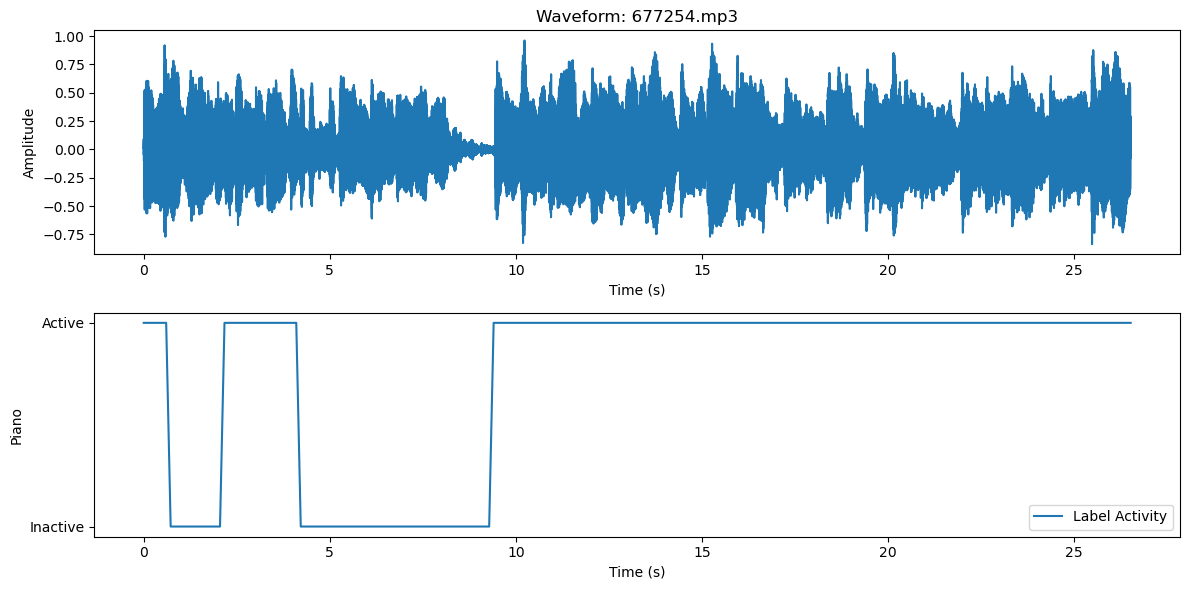
\includegraphics[width=0.75\linewidth]{output1.png}
  \caption{Analysis of the mapped class using the labeling function.}
  \label{fig1}
\end{figure}
\pagebreak

\textbf{231710.mp3:}
This file was annotated five times with the descriptions "rhythmic drumming", "a man is talking nearby". The beginning of the file includes a drum part for 5 seconds and then a two men begin to have a conversation. The original captions match the free-text annotations. The labeling function has correctly identified the partitions of the file as "Speech" and "Drums" (for a detailed graph \autoref{fig2}). All sound events in the file are clearly audible.

\begin{figure}[H]
  \centering
  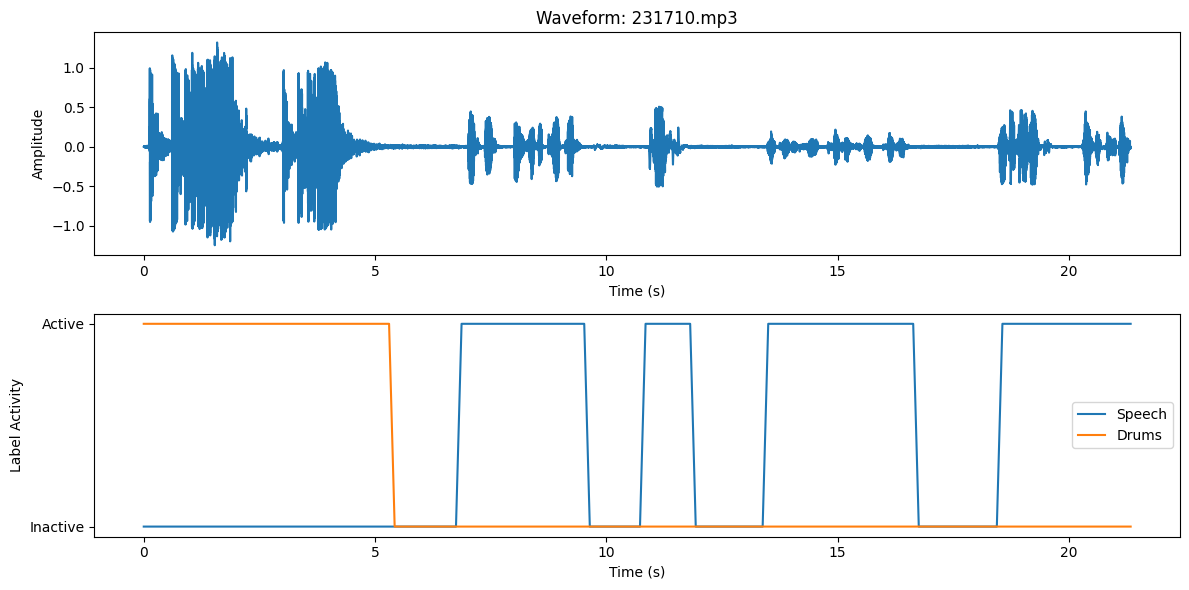
\includegraphics[width=0.75\linewidth]{output2.png}
  \caption{Using the waveform to assess if the labels were correctly identified.}
  \label{fig2}
\end{figure}

\textbf{TODO: 1b, 1c}

\section{Data Split}
\label{sec:data_split}
We have decided to use 80 \% of the data for training (so that the model has enough examples to generalize) with 10\% for validation (to reduce overfitting) and 10\% for testing (to estimate the model's unbiased performance). The training set was used for cross-validation and the validation set was used for fine-tuning the hyperparameters. The remaining 10\% was used to evaluate the model's performance.

Yes, there are potential risks for information leakage, namely, if the features in the training set are highly correlated with the labels of the test set, this could cause feature leakage. Avoiding to use features from the test set could prevent this type of leakage. 

There could also be issues with multiple recordings of the same subject such as "wind" where the model could rely heavily on these subject-specific aspects of the data. One way to address this would be to split the data in such a way that the samples containing information about the same subject are either only in the test set or the training set. 

Semantic similarity of class labels could be another issue where the annotation embeddings could have high similarity for certain classes and text embeddings. 



\section{Audio Features}
\label{sec:audio_features}
During the initial phase of the project, we performed exploratory data analysis to identify some important features. Building on those insights, we applied Principal Component Analysis (PCA) to our 768-dimensional feature embeddings, reducing them to just 100 principal components that together explain approximately 90\% of the total variance. This reduces the computational costs significantly, while maintaining the bulk of the information needed to train our models.

\section{Evaluation}
\label{sec:evaluation}
To compare hyperparameter settings and evaluate our models, we use the balanced accuracy score. Since we are dealing with imbalanced data (not all classes are equally distributed), it prevents a model from getting a good score simply by favoring the majority class. 
\\
$$\text{Balanced Accuracy} = \frac{1}{2} \left(\frac{\mathrm{TP}}{\mathrm{TP} + \mathrm{FN}} + \frac{\mathrm{TN}}{\mathrm{TN} + \mathrm{FP}} \right)$$
\\\\
We implemented a simple baseline classifier that always predicts the majority class by default. \\ 
For example, when asking if 'drums' occur in '231710.mp3' (see \ref{fig2}), the baseline predicts 0 because the label is inactive most of the time. Using plain accuracy this already achieves about 75\%, but this simply captures the imbalance between “no-drums” and “drums”. In contrast, balanced accuracy gives equal weight to the true-positive rate and the true-negative rate. This prevents a classifier from appearing strong merely by favoring the dominant class, getting a better evaluation when one class is less frequent.

\section{Experiments}
\label{sec:experiments}
To reduce computational efforts, we only use a subset of samples during hyperparameter tuning. This allows us to vary the values of parameters and compare the results to find a good combination, but keep the training time relatively low. For Classifiers with multiple parameters we perform a grid search using all possible combinations.

\subsection{K-Nearest Neighbors Classifier}
Because each sound event is either present or absent, we treat each label as its own binary classification task. We apply a K-nearest Neighbors (KNN) classifier independently to each label and run repeated evaluations to identify the best hyperparameters. In this setup, the number of $k$ neighbors is crucial: choosing $k$ too small makes the model too complex and prone to overfitting, while a very large $k$ leads to underfitting.

\begin{figure}[H]
  \centering
  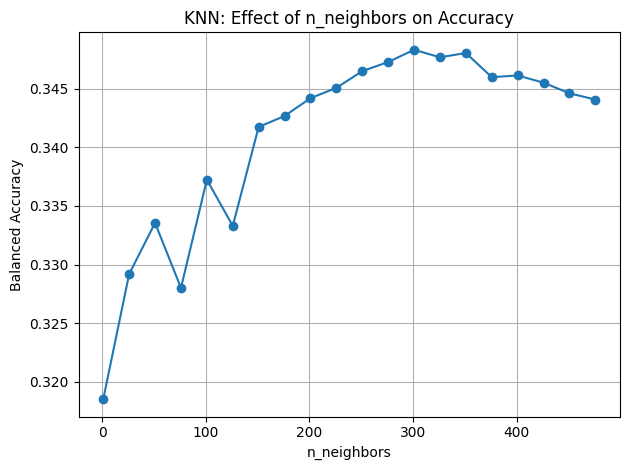
\includegraphics[width=0.30\linewidth]{knn_performance.png}
  \caption{KNN accuracy for different k}
  \label{fig_knn}
\end{figure}

\subsection{Decision Tree}
A Decision Tree is another straightforward approach for our binary classification tasks. Like with KNN, we perform a hyperparameter search to find the ideal settings. Increasing \textit{max\_depth} allows deeper nested decisions and improves the fit on the training data but also raises the risk of overfitting. To counteract that problem, we can also raise \textit{min\_samples\_split} and \textit{min\_samples\_split}, which forces each node or leaf to have a minimum number of samples before the split can occur. Despite this regularization, our best single-tree model still performs worse than the KNN on our noisy data. The peak balanced accuracy was only 0.28.

\subsection{Random Forest Classifier with Multi-Label Classification}
Since we have multiple classes in our data, we also evaluated a Random Forest classifier on all 58 labels and observed a significant improvement over both KNN and a single Decision Tree. Using 58 trees (\textit{n\_estimators=58}), a maximum depth of 30, min. samples per split of 10 and the “entropy” criterion, the model achieved a balanced accuracy score of 0.6472. This result shows that Random Forests combined with the Multi-Output Classifier works best with our data.\\
These hyperparameters were then applied to train our final model on the full training dataset, and its predictions were evaluated across all classes. (see \ref{sec:analyzing_predictions})

\pagebreak
\section{Analyzing Predictions}
\label{sec:analyzing_predictions}
After we have found the "best" hyperparameters, we trained our model on the full training set (see \ref{sec:data_split}). \\
At first the predictions of the model seemed pretty disappointing. The model did not capture different sound events or predicted the wrong labels. We assumed it would only work for simple examples:

\begin{figure}[H]
  \centering
  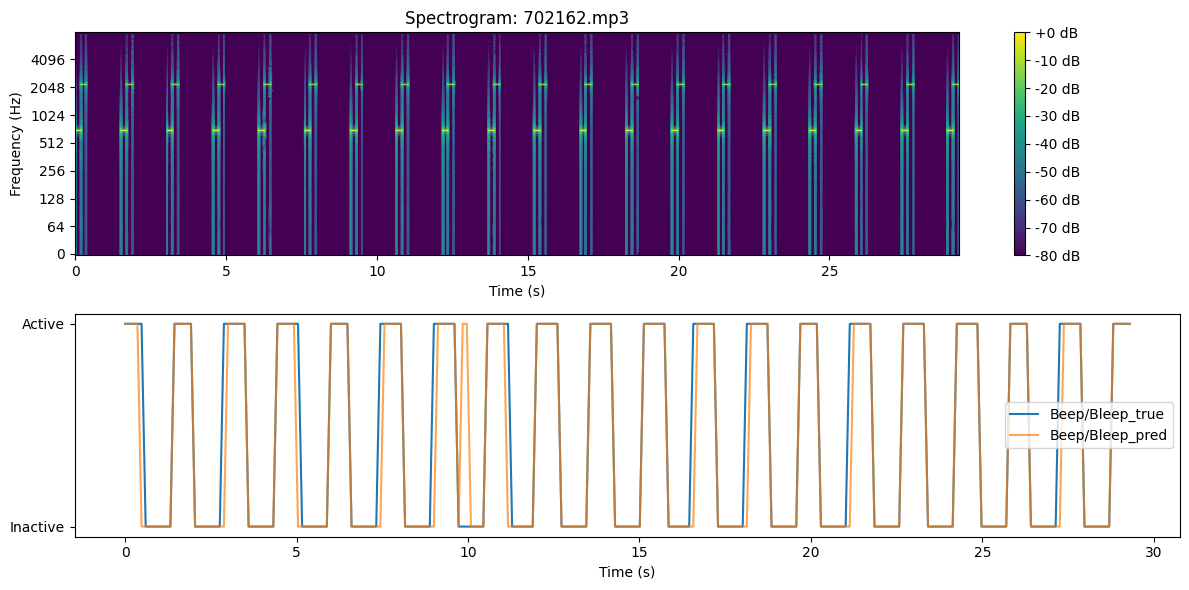
\includegraphics[width=0.75\linewidth]{702162_pred.png}
  \caption{702162.mp3: Ground Truth vs Prediction}
  \label{fig3}
\end{figure}

The beep sounds in '702162.mp3' are clearly audible and it's a pretty unique sound. So we would expect the model to be able to capture this kind of sound event and indeed the predictions are pretty accurate. \\
However, after further investigation and comparing the true annotations with our prediction we found many samples where the model actually performed better than the annotators themselves. This also applies for more complex sound events. Lets look at two examples:

\begin{figure}[H]
  \centering
  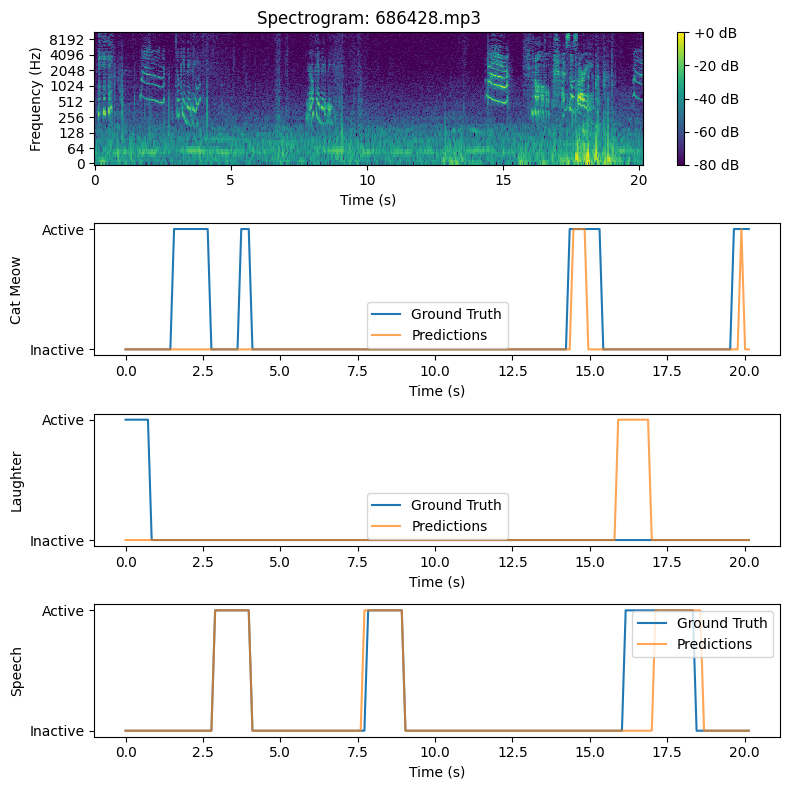
\includegraphics[width=0.6\linewidth]{686428_pred.png}
  \caption{686428.mp3: Ground Truth vs Prediction}
  \label{fig4}
\end{figure}

Despite the fact that the model misses the first occurences of the meowing cat, it captured the talking person very accurately. When we listen to the audio file, we can clearly hear the person laughing at around 16s. This was captured by our model, but was described as 'speech' by the annotator. 

\begin{figure}[H]
  \centering
  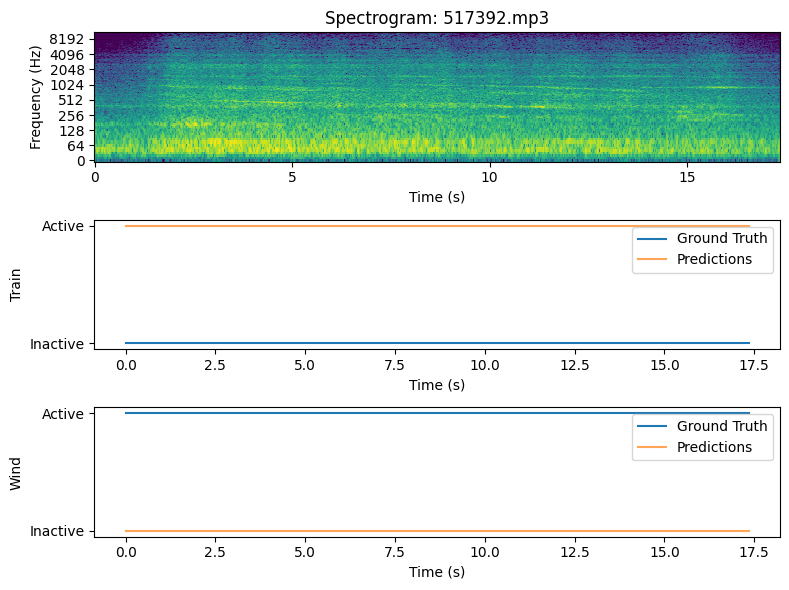
\includegraphics[width=0.6\linewidth]{517392_pred.png}
  \caption{517392.mp3: Ground Truth vs Prediction}
  \label{fig5}
\end{figure}

This time, the Ground Truth label is completely wrong. The file definitely contains the sound of a passing train, which was correctly identified by the model. \\

Overall we see that the performance is not that bad. Some sound events are pretty hard to distinguish and our model completely fails, but there are also many examples where the performance is actually very good.
\\\\
One of the biggest problems we encountered was that the predictions were very fragmented - short spikes with activity/inactivity of different labels. To mitigate this problem we should definitely consider smoothing the predictions as a postprocessing step. One simple solution could be a majority voting for a certain audio window (multiple combined audio frames).

\end{document}